% \begin{figure}[t!]
% 	% \vspace{-12pt}
% 	 \renewcommand{\arraystretch}{0.4}
% 	\centering
% 	\resizebox{1\columnwidth}{!}{%
% 	\begin{tabular}{@{}c@{\hskip .1cm}c@{\hskip .1cm}c@{}}
% 	    {\small (a) Input Frame} & {\small (b) w/ Schedule} & {\small (c) wo/ Schedule} \\
%     	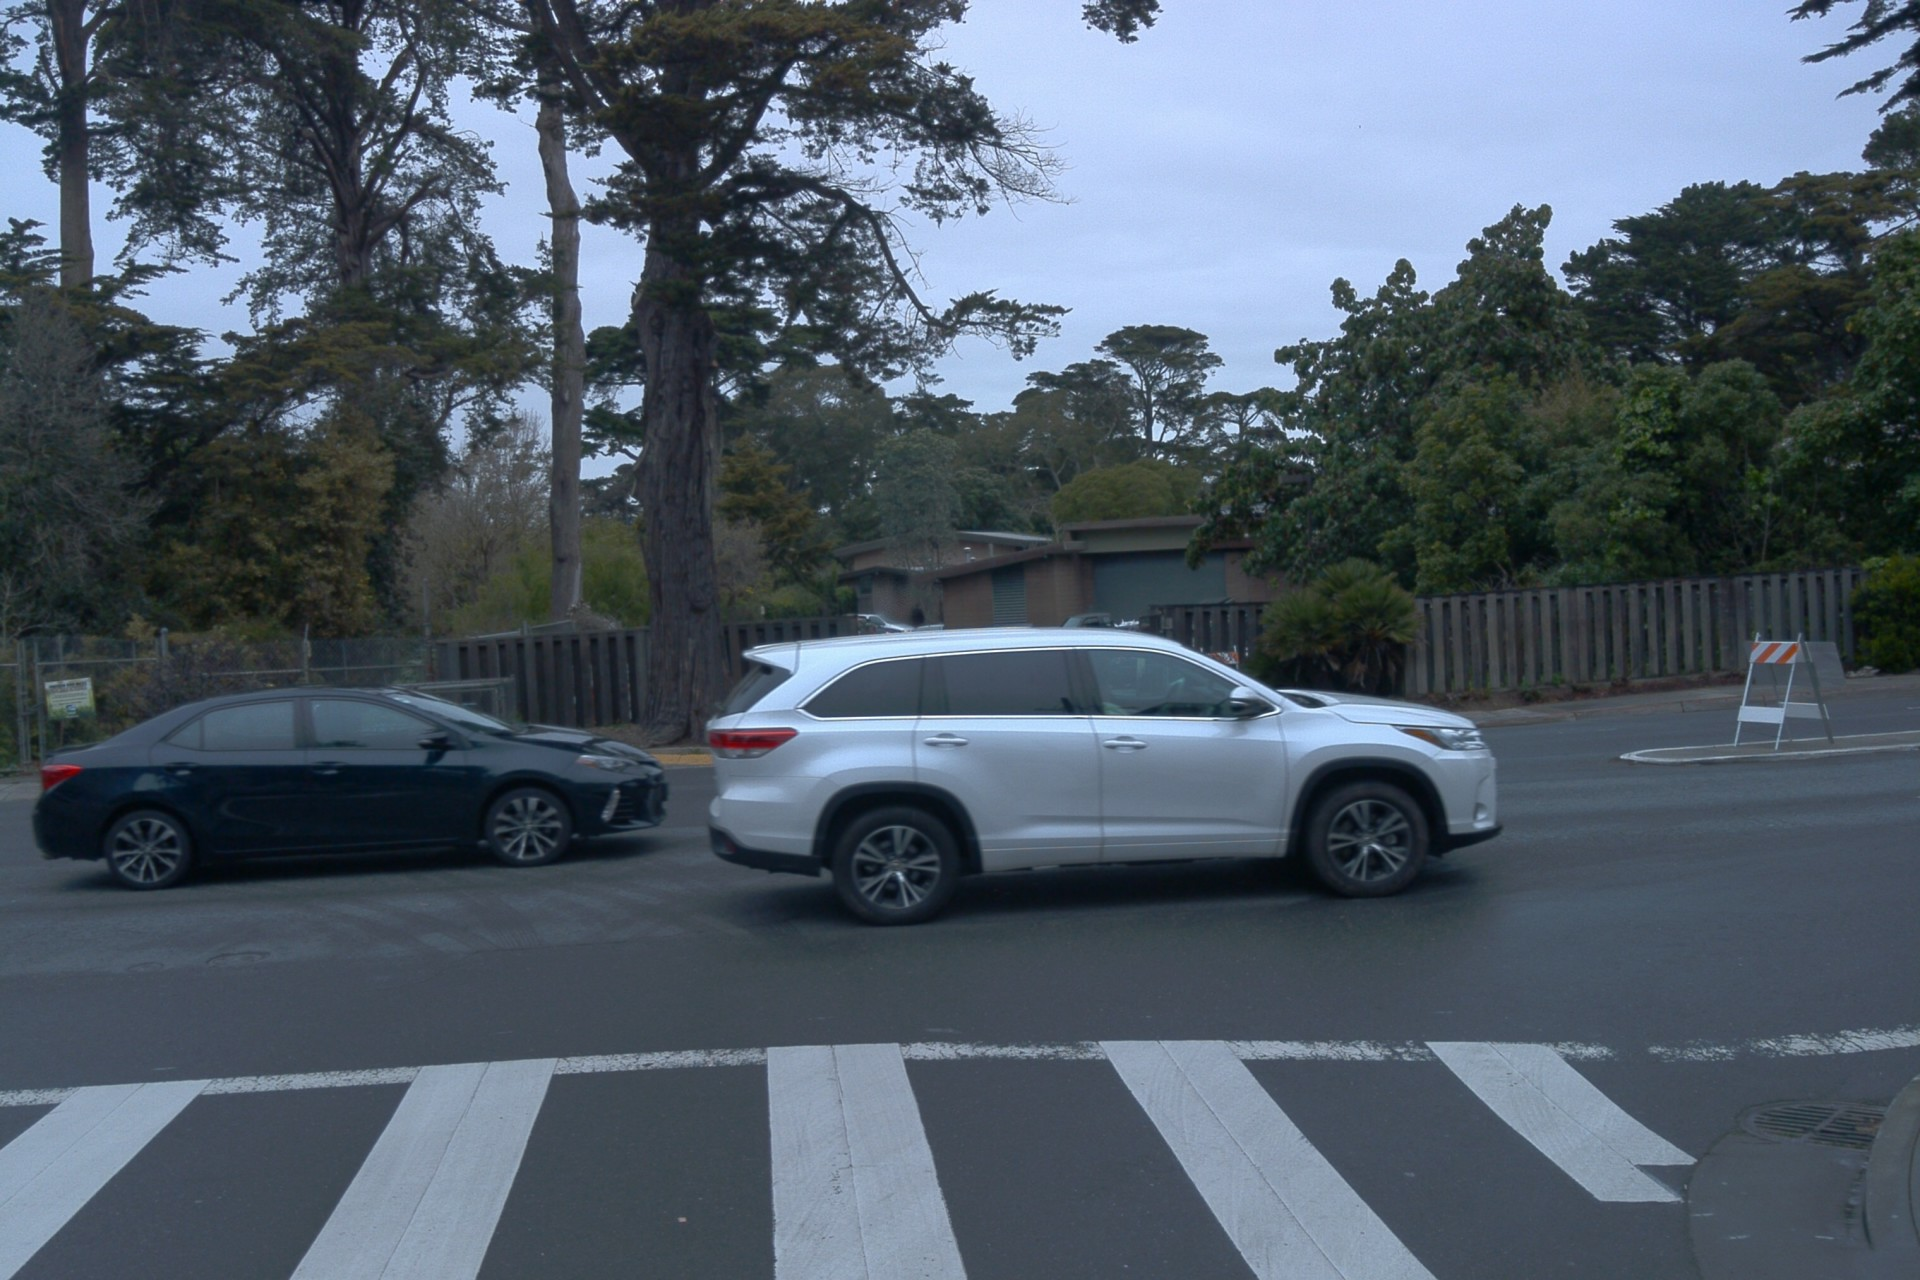
\includegraphics[width=.31\columnwidth, trim={0cm 0cm 0cm 0cm},clip]{fig/rebuttal_optimization/gt/11_102_gt.png}&
%     	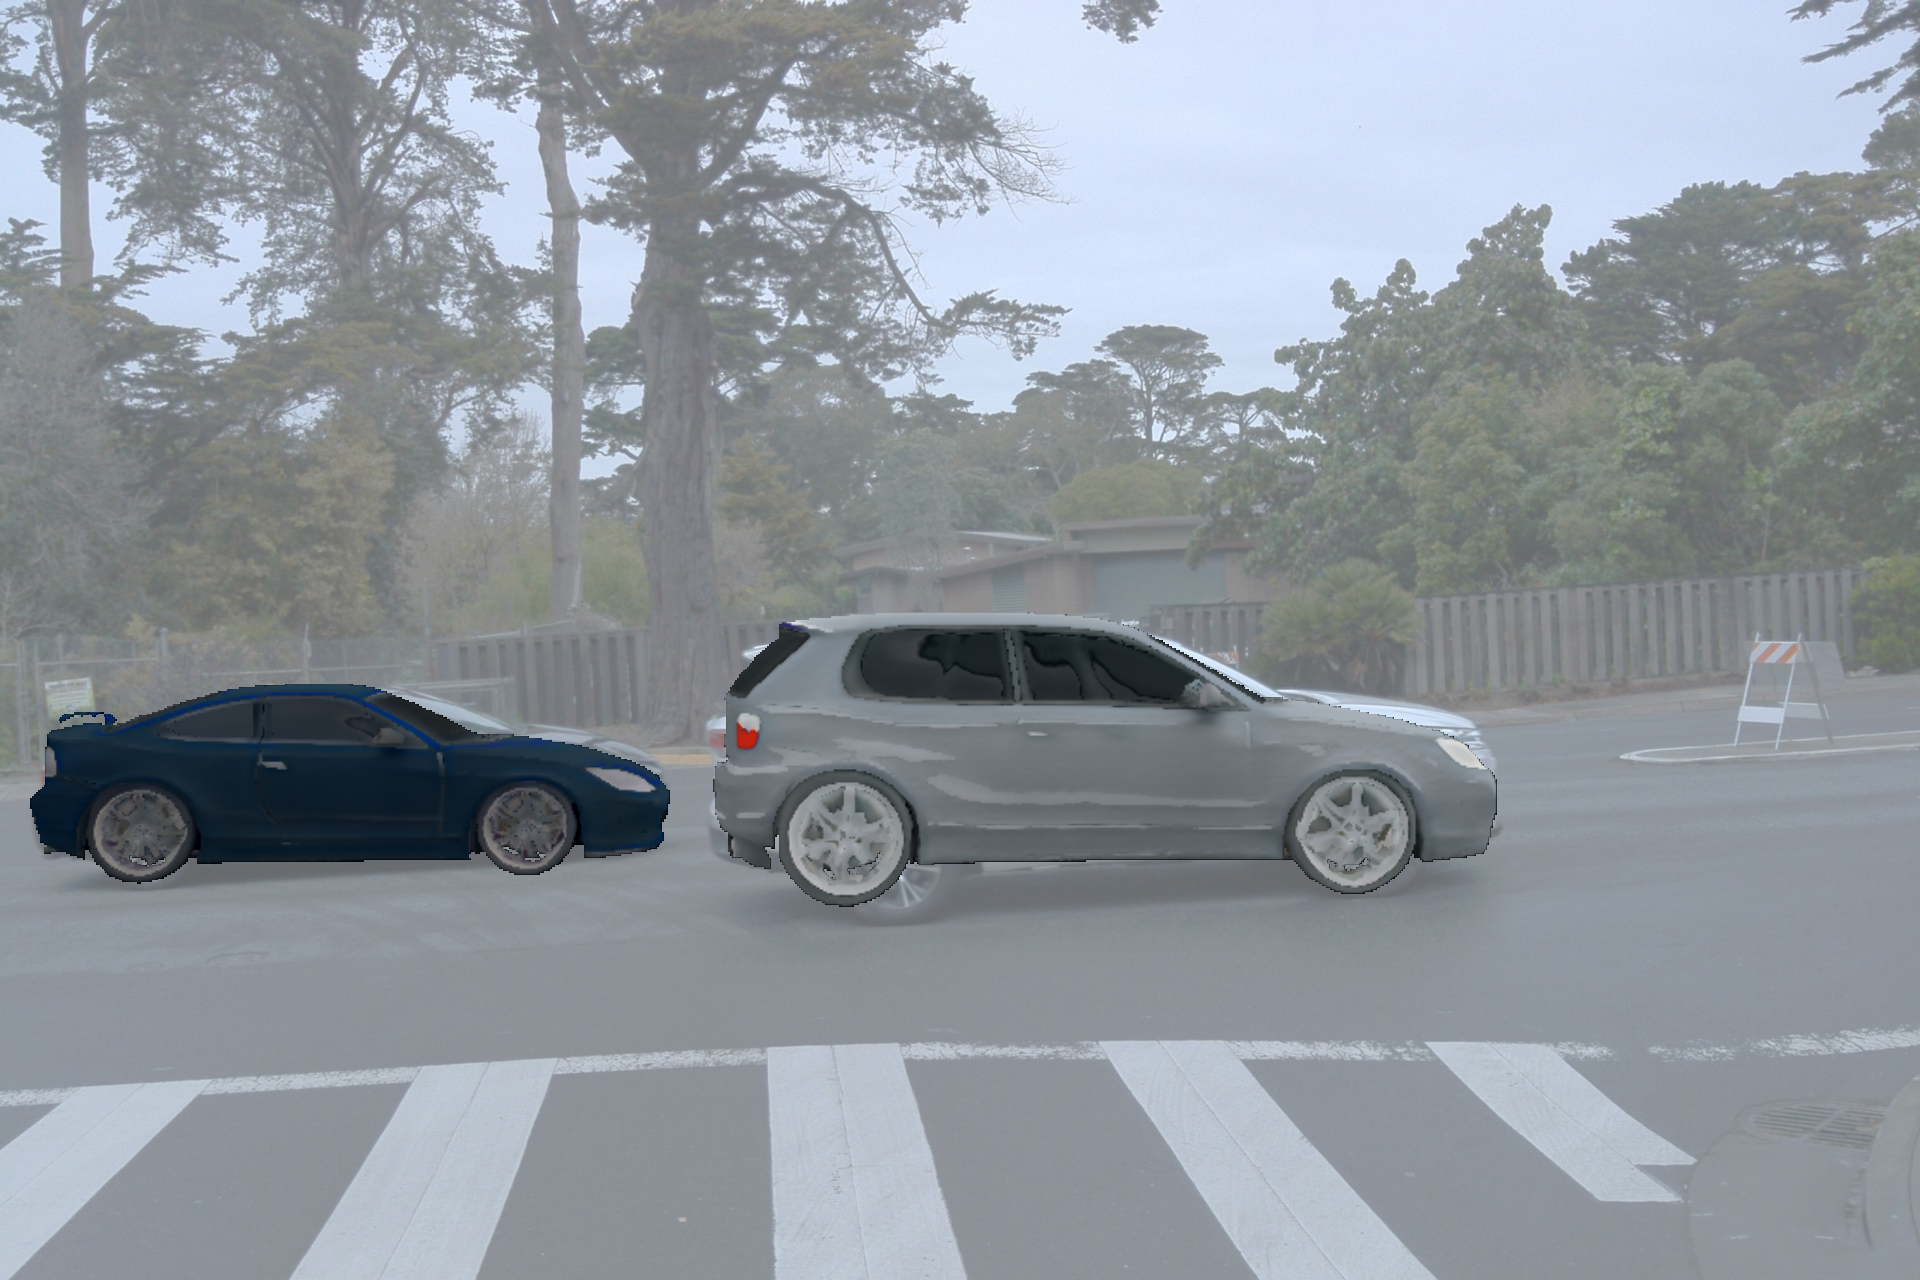
\includegraphics[width=.31\columnwidth, trim={0cm 0cm 0cm 0cm},clip]{fig/rebuttal_optimization/sched/11_102_sched.png}&
%     	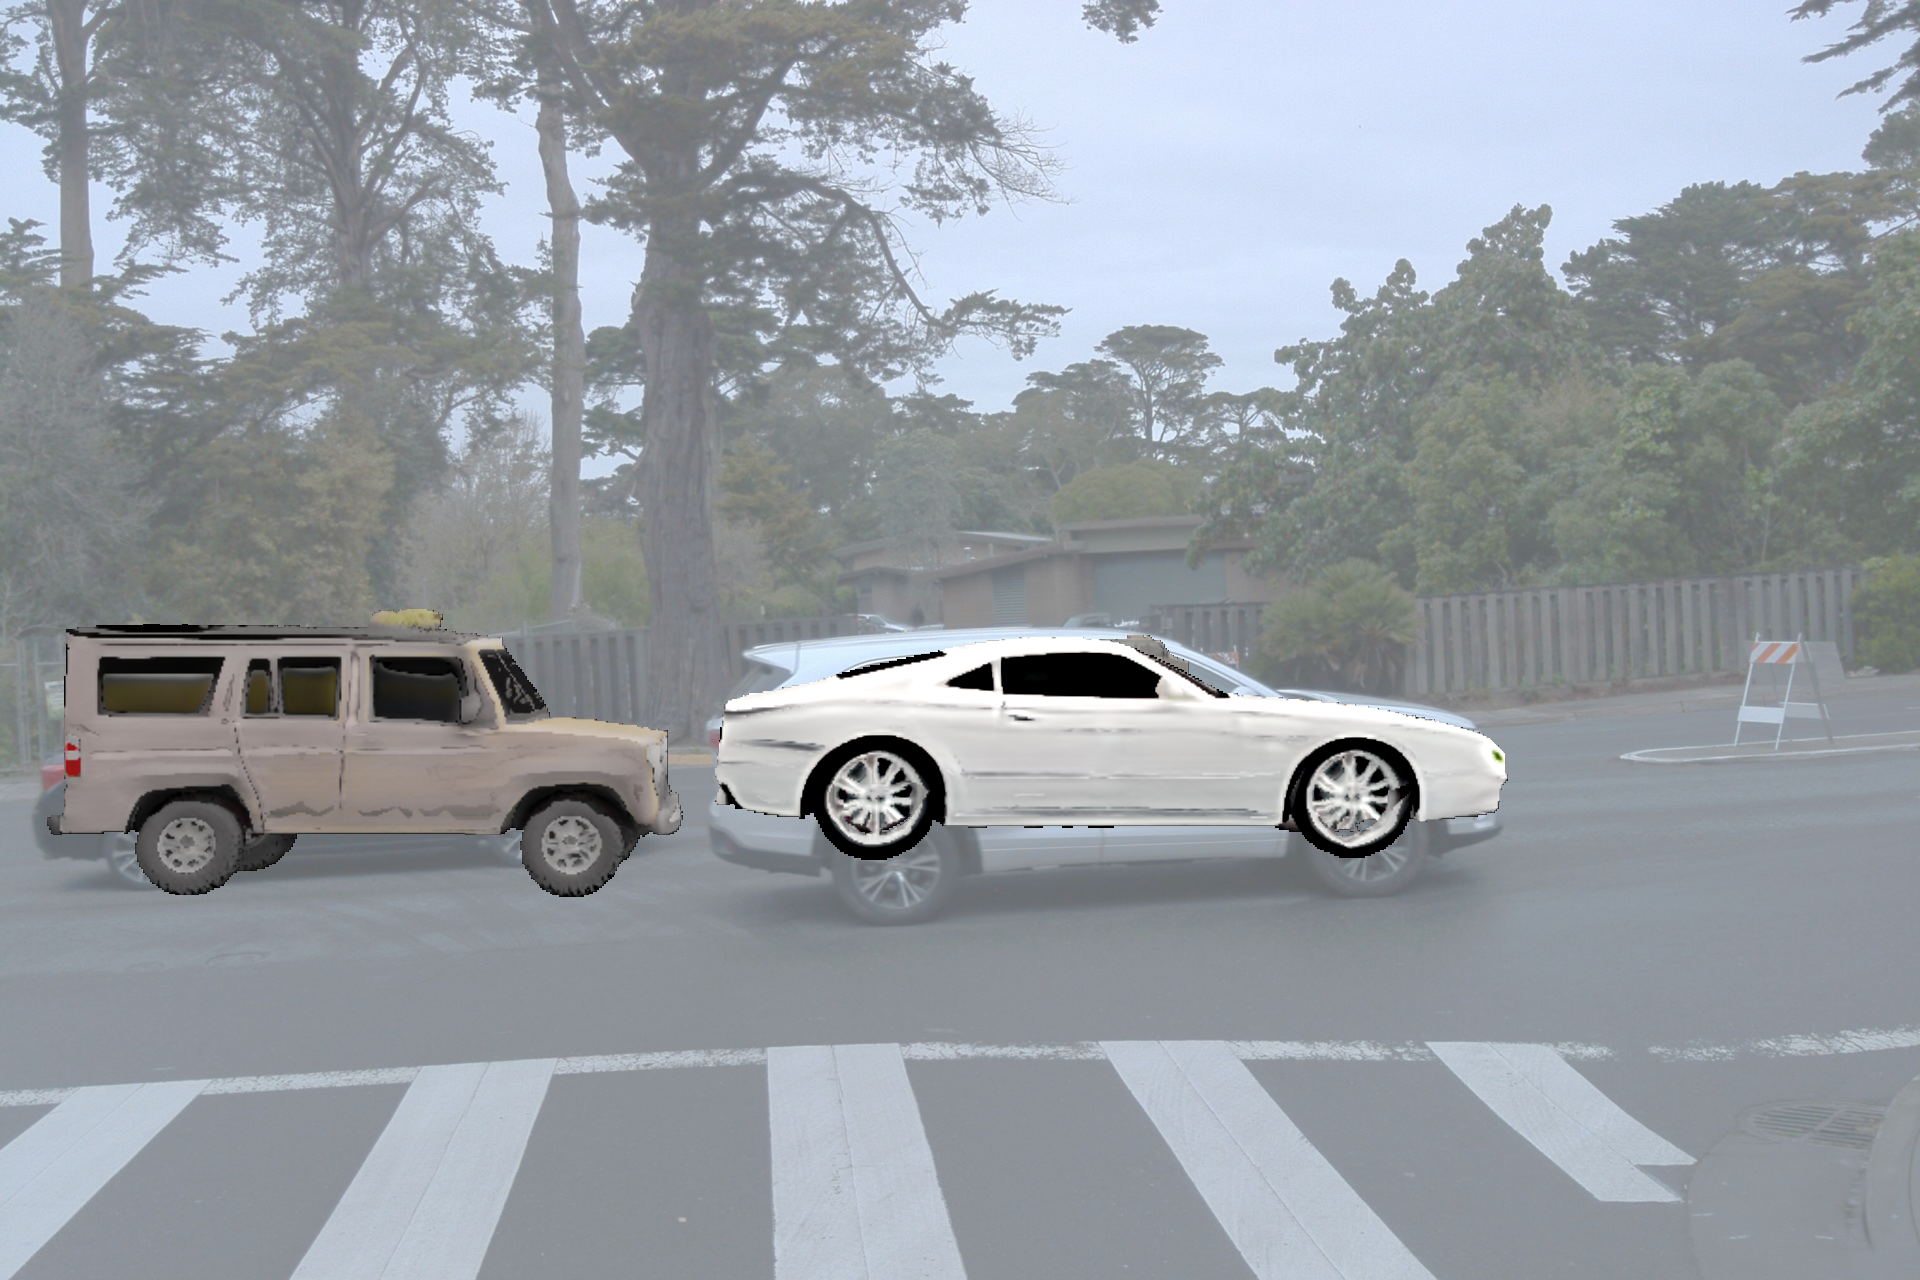
\includegraphics[width=.31\columnwidth, trim={0cm 0cm 0cm 0cm},clip]{fig/rebuttal_optimization/no_sched/11_102_no_sched.png}\\
%     	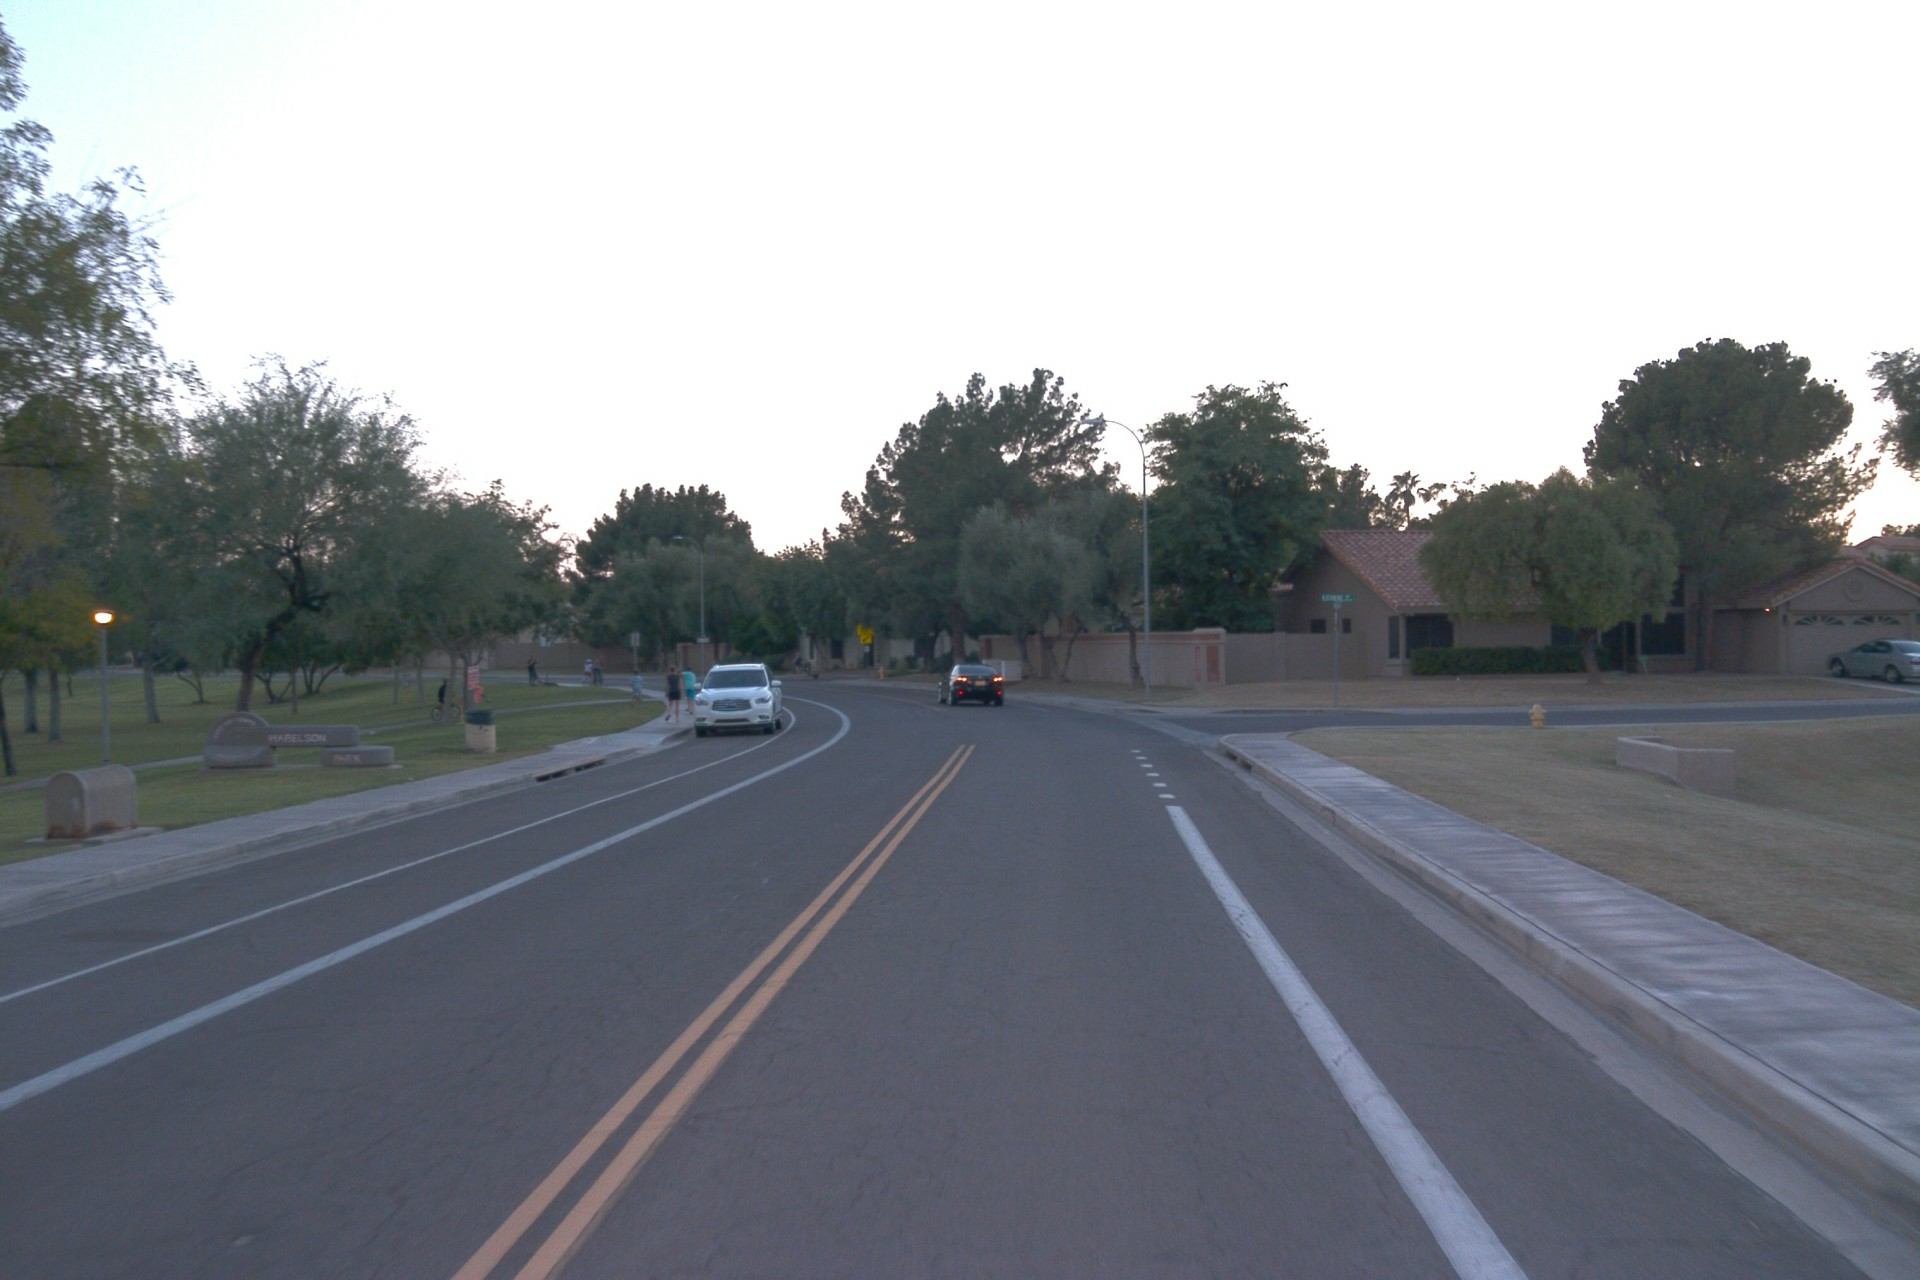
\includegraphics[width=.31\columnwidth, trim={22cm 17cm 30cm 18cm},clip]{fig/rebuttal_optimization/gt/82_60_gt_img.png}&
%     	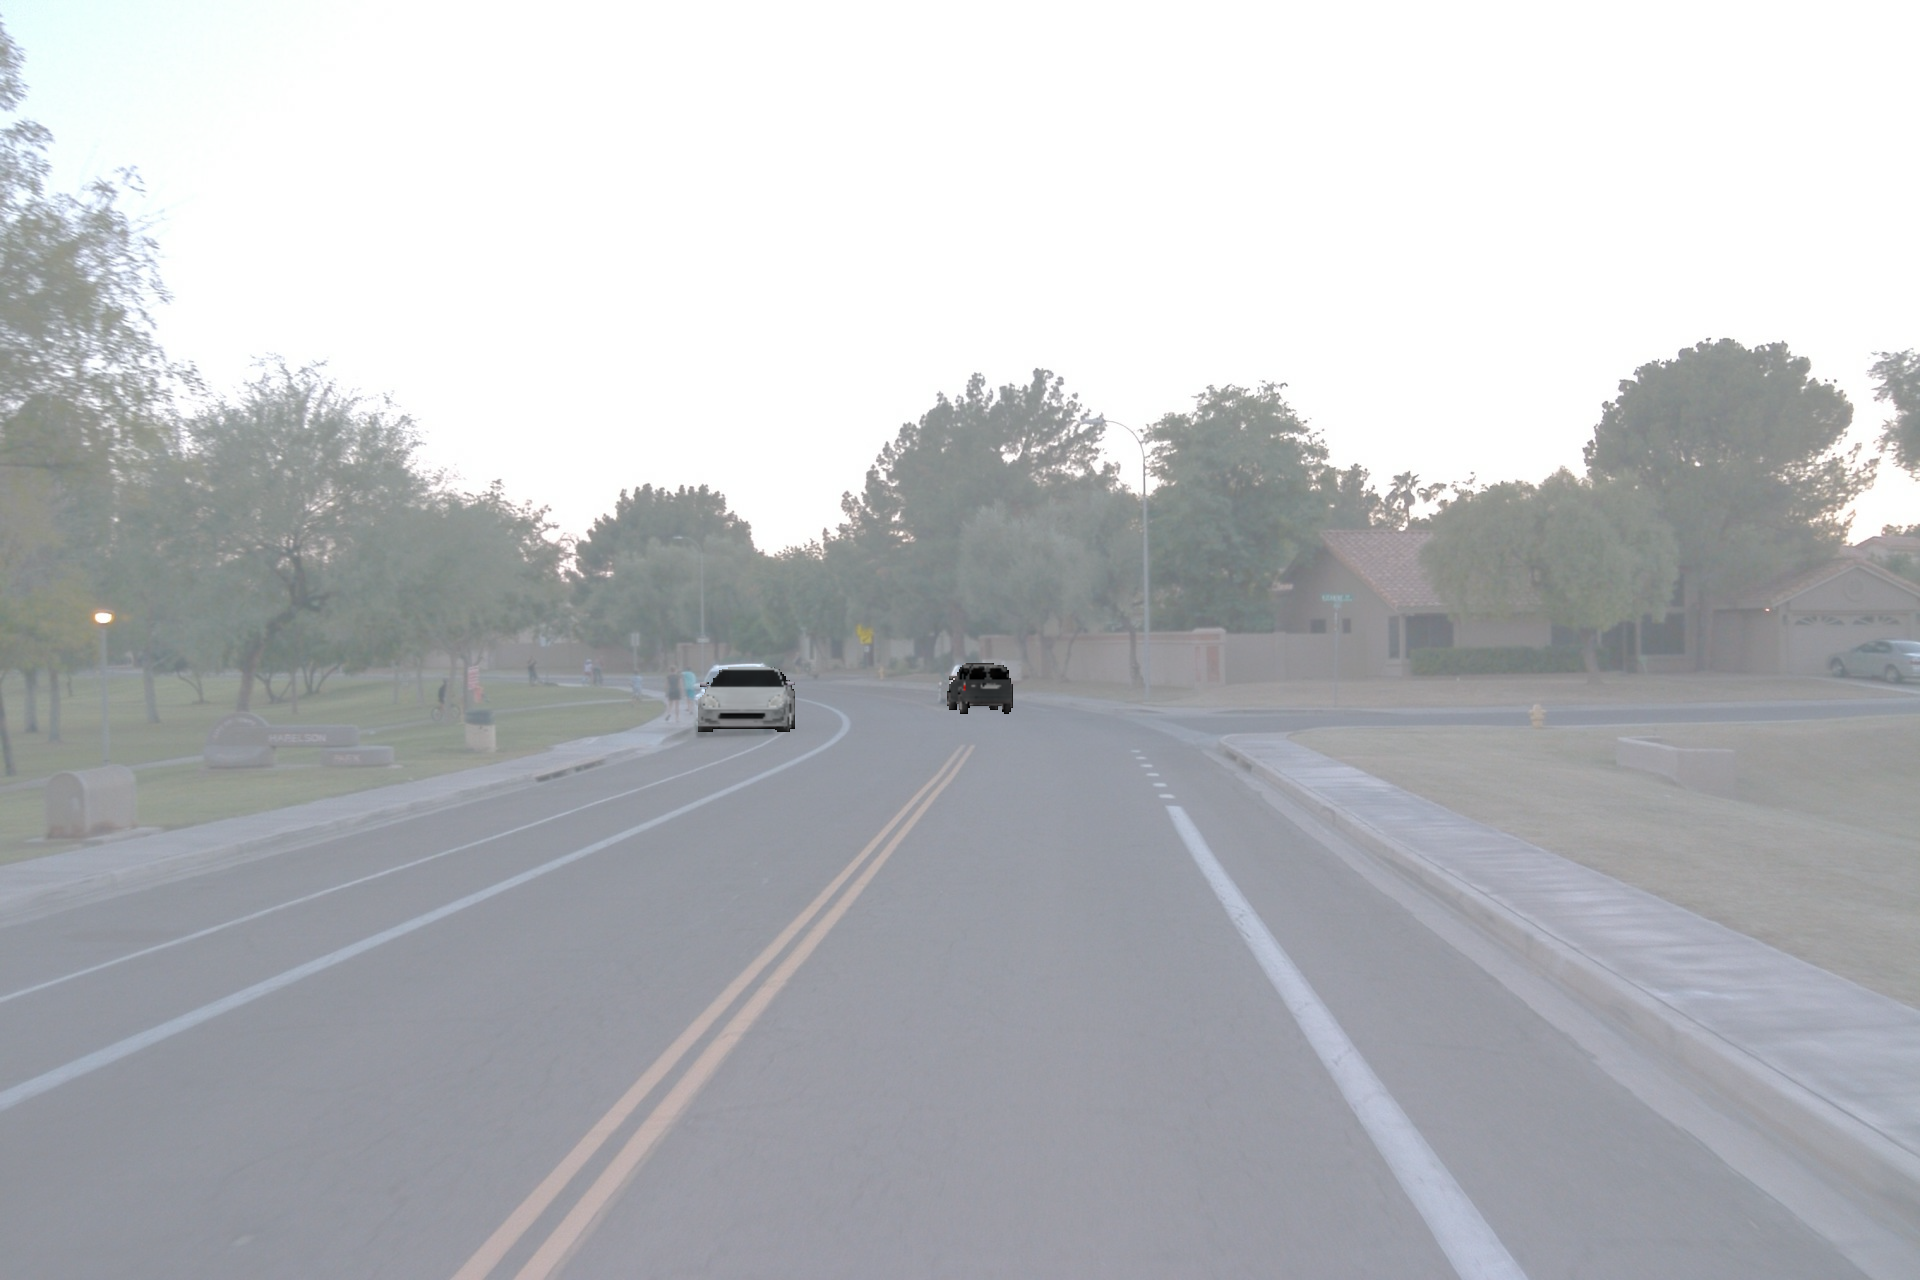
\includegraphics[width=.31\columnwidth, trim={22cm 17cm 30cm 18cm},clip]{fig/rebuttal_optimization/sched/82_60_shed.png}&
%     	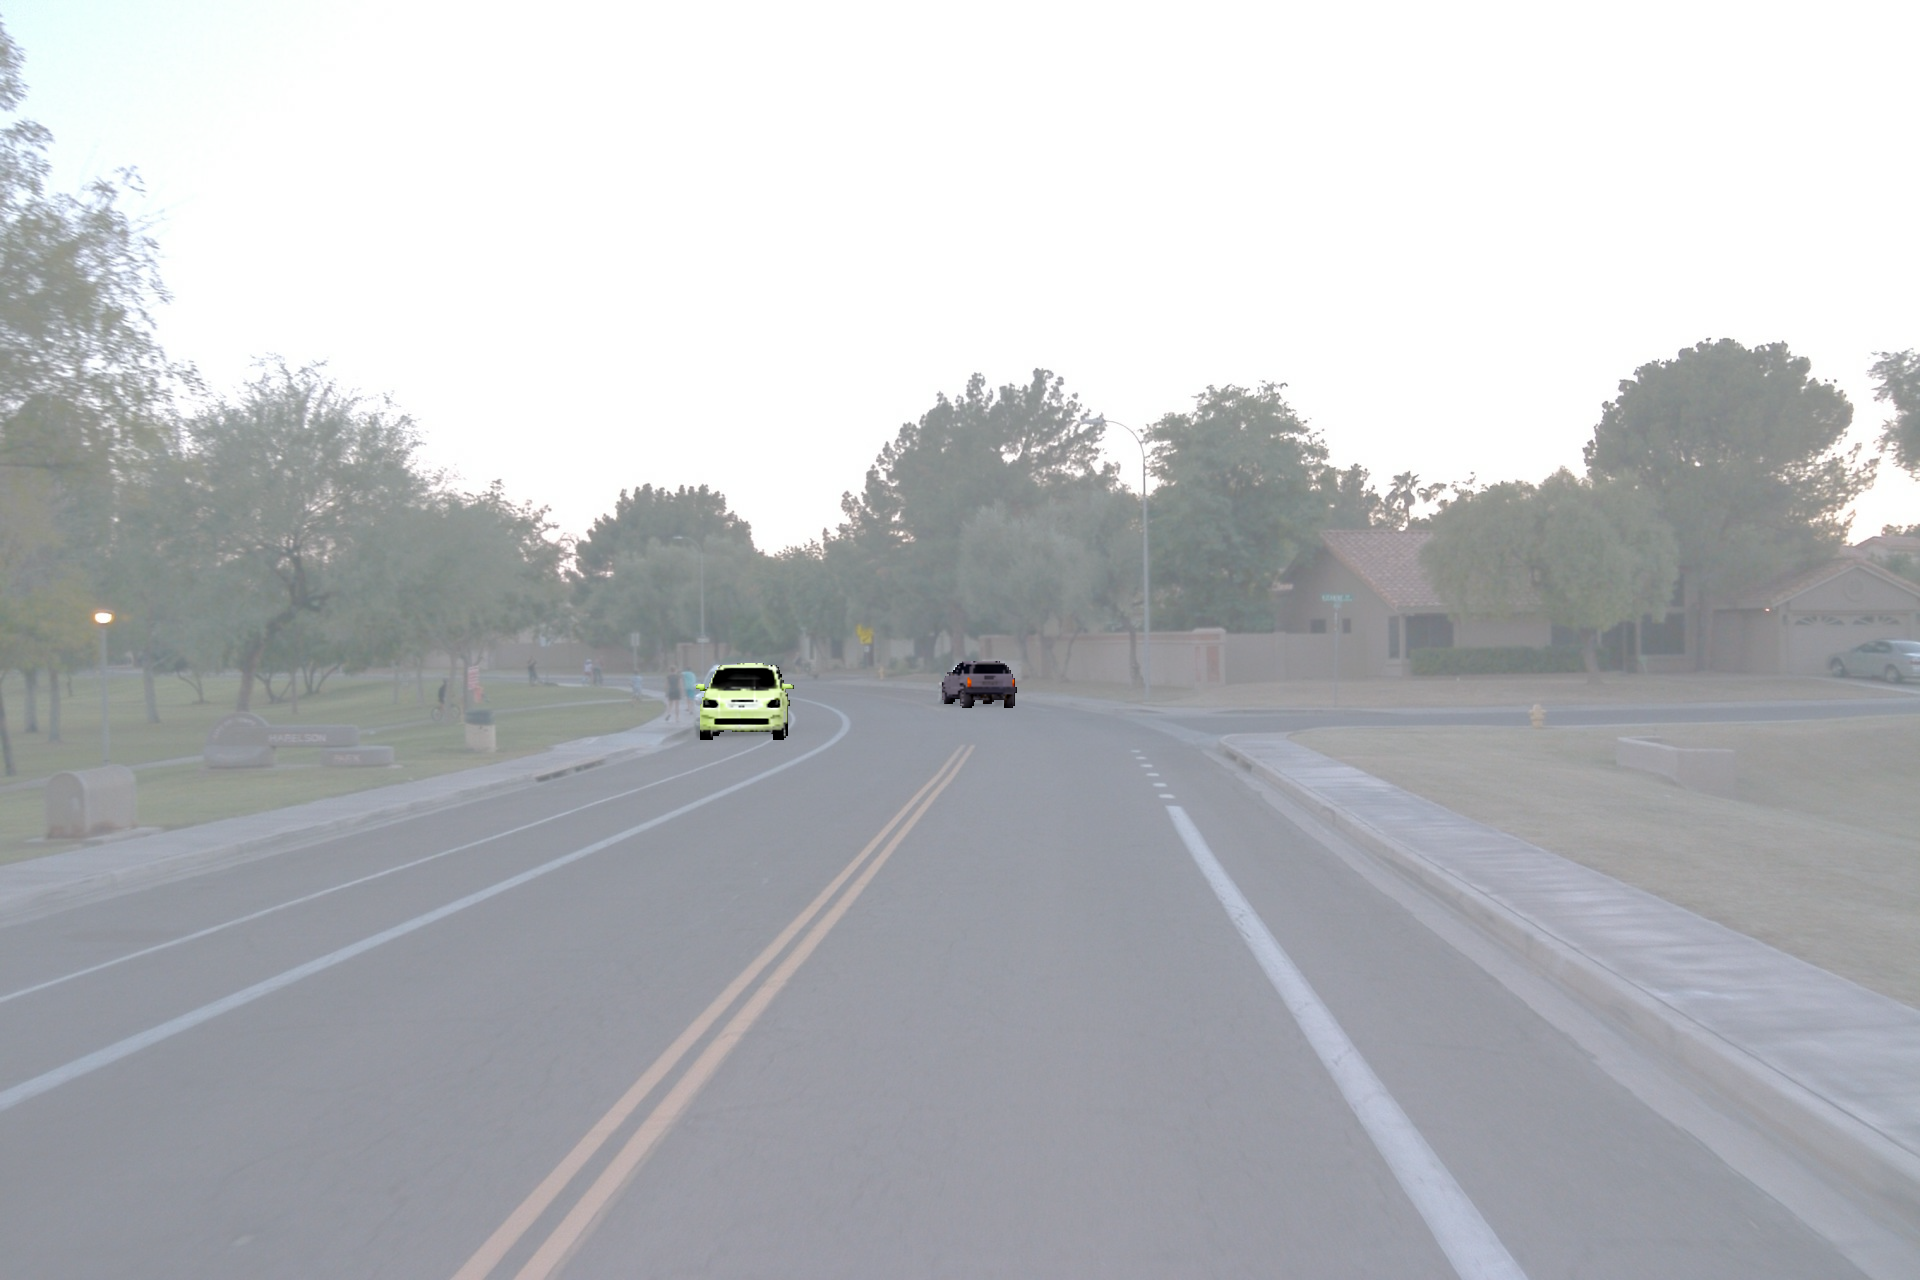
\includegraphics[width=.31\columnwidth, trim={22cm 17cm 30cm 18cm},clip]{fig/rebuttal_optimization/no_sched/82_60_no_shed.png}\\
%     \end{tabular}}\vspace*{-6pt}
% 	\caption{\todo{Make split figure} \textbf{Effect of Optimization Schedule.} (a) observed image, (b) optimized generations using the proposed schedule (see 3.1 \& 3.3), (c) optimized generations using no schedule.
%  % , i.e. such that texture codes, shape codes, rotations, translations, and scales are all simultaneously optimized. The ground truth images are faded to show our rendered objects clearly. 
%     % The bottom row shows images zoomed in to clearly show our rendered objects.
%     % Our schedule allows for more stable optimization, with rendered objects more closely resembling the observed ones. 
%  } 
% 	\label{fig:opt_scheduler}
% 	% \vspace{-8pt}
% \end{figure}


\begin{figure}[t!]
% \vspace{-12pt}
\renewcommand{\arraystretch}{0.4}
\centering
% \resizebox{1\columnwidth}{!}{%
\begin{tabular}{@{}c@{\hskip .1cm}c@{\hskip .1cm}c@{\hskip .1cm}c@{\hskip .1cm}c@{\hskip .1cm}c@{}}
    \multicolumn{2}{c}{(a) Input Frame} & \multicolumn{2}{c}{(b) Full (ours)} & \multicolumn{2}{c}{(c) \underline{No Schedule}} \\
    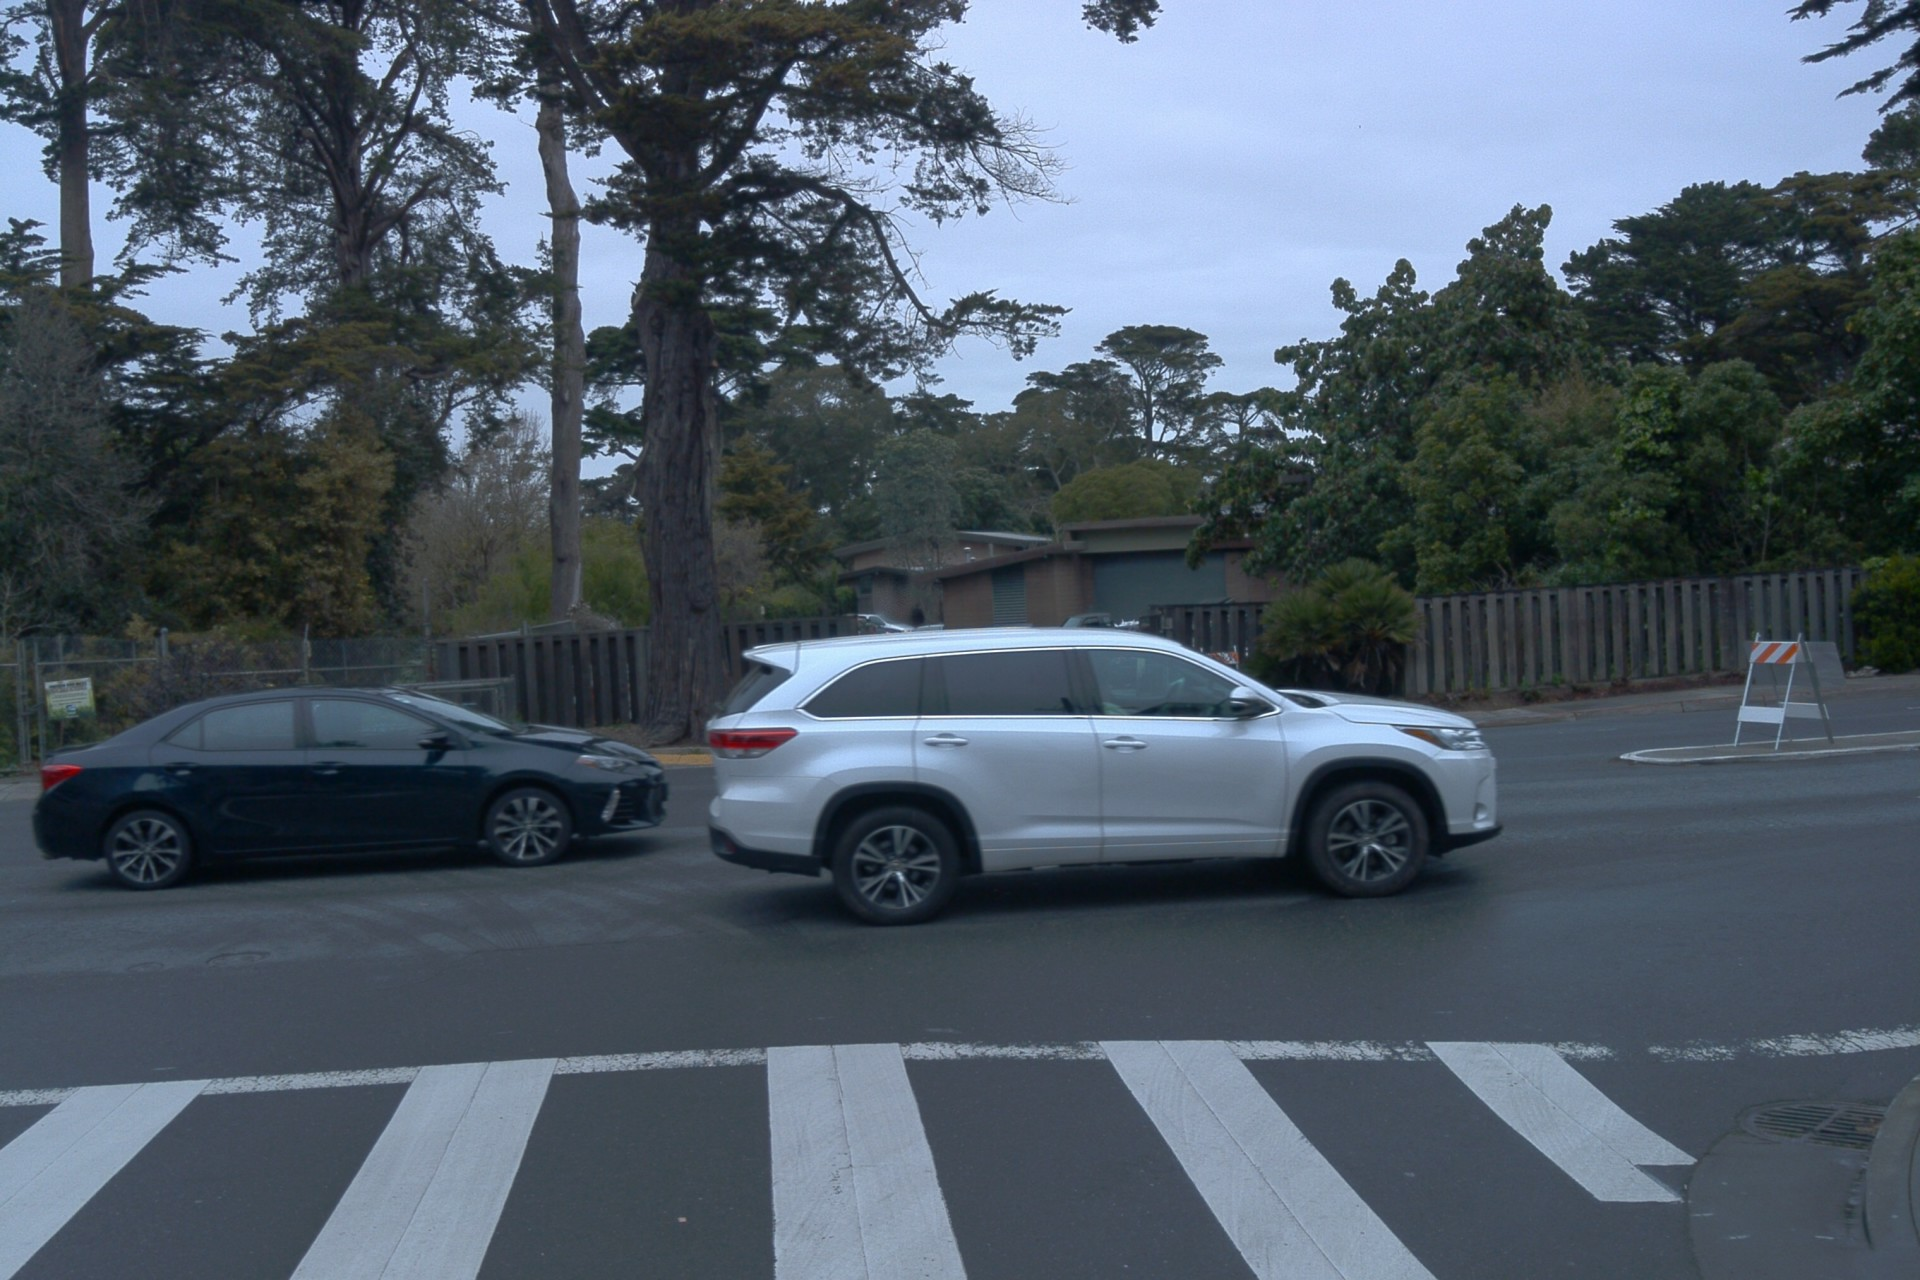
\includegraphics[width=.16\columnwidth, trim={0cm 0cm 0cm 0cm},clip]{fig/rebuttal_optimization/gt/11_102_gt.png}&
    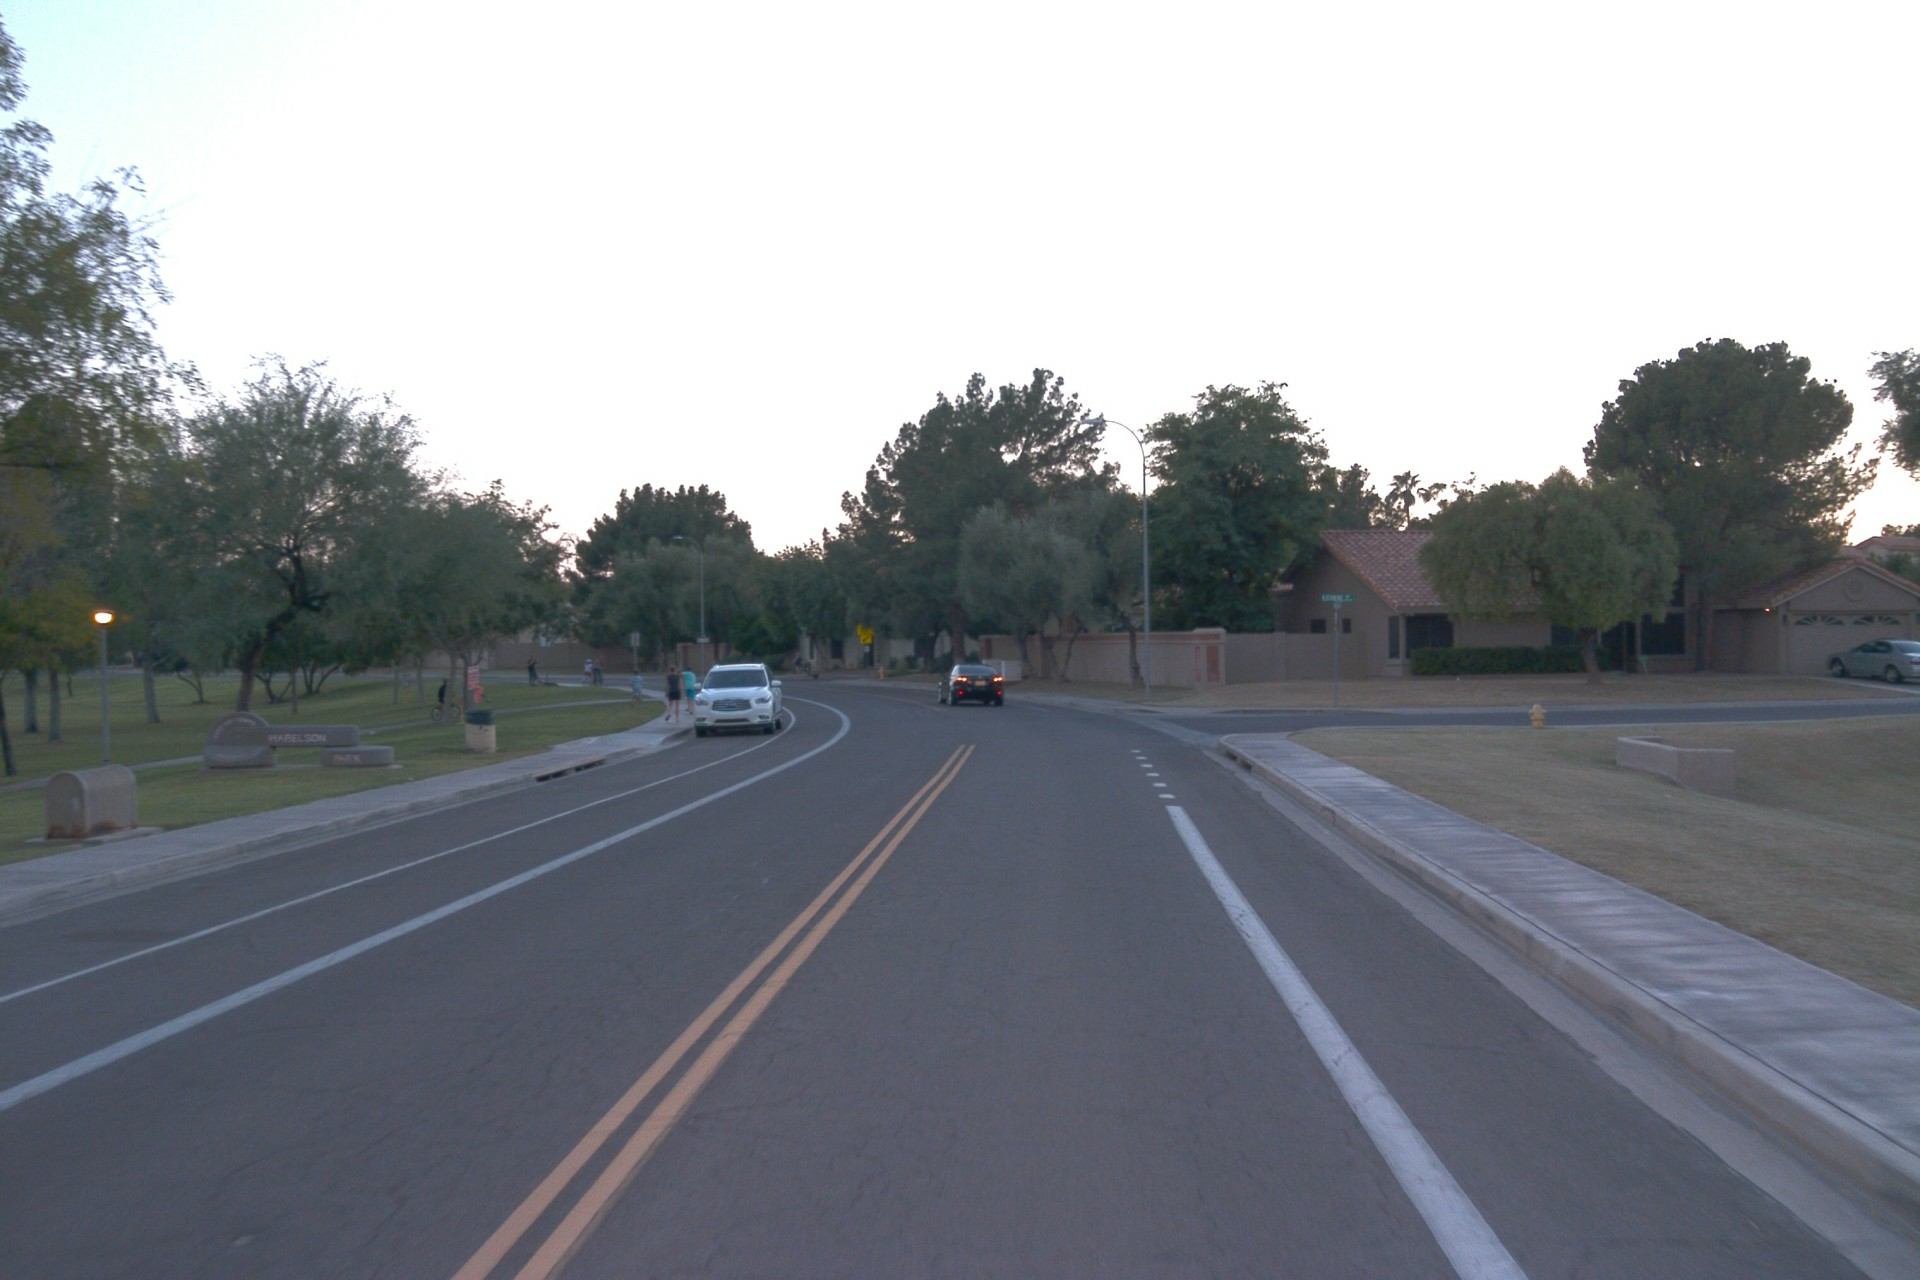
\includegraphics[width=.16\columnwidth, trim={22cm 16.68cm 30cm 18cm},clip]{fig/rebuttal_optimization/gt/82_60_gt_img.png}&
    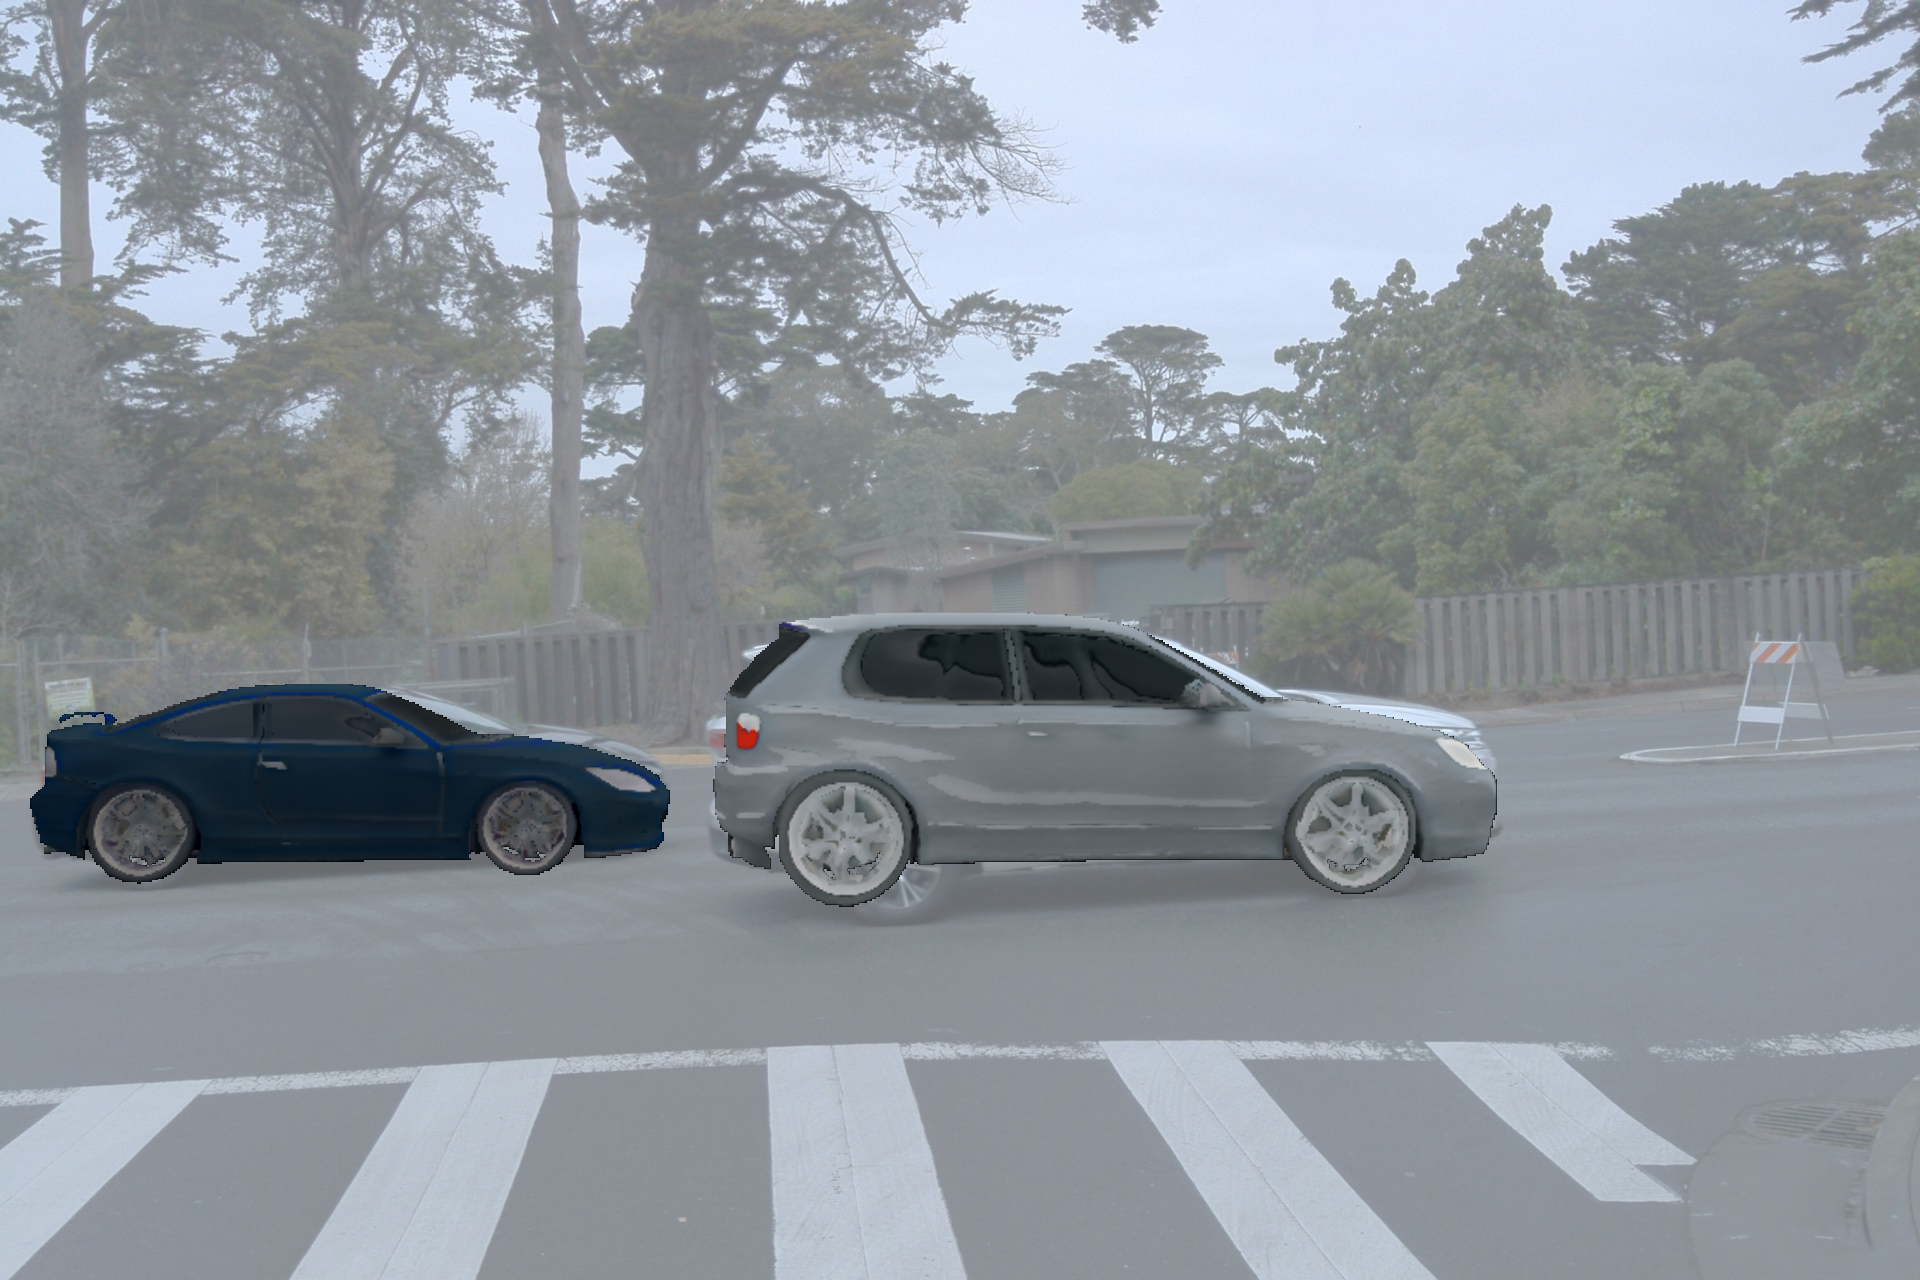
\includegraphics[width=.16\columnwidth, trim={0cm 0cm 0cm 0cm},clip]{fig/rebuttal_optimization/sched/11_102_sched.png}&
    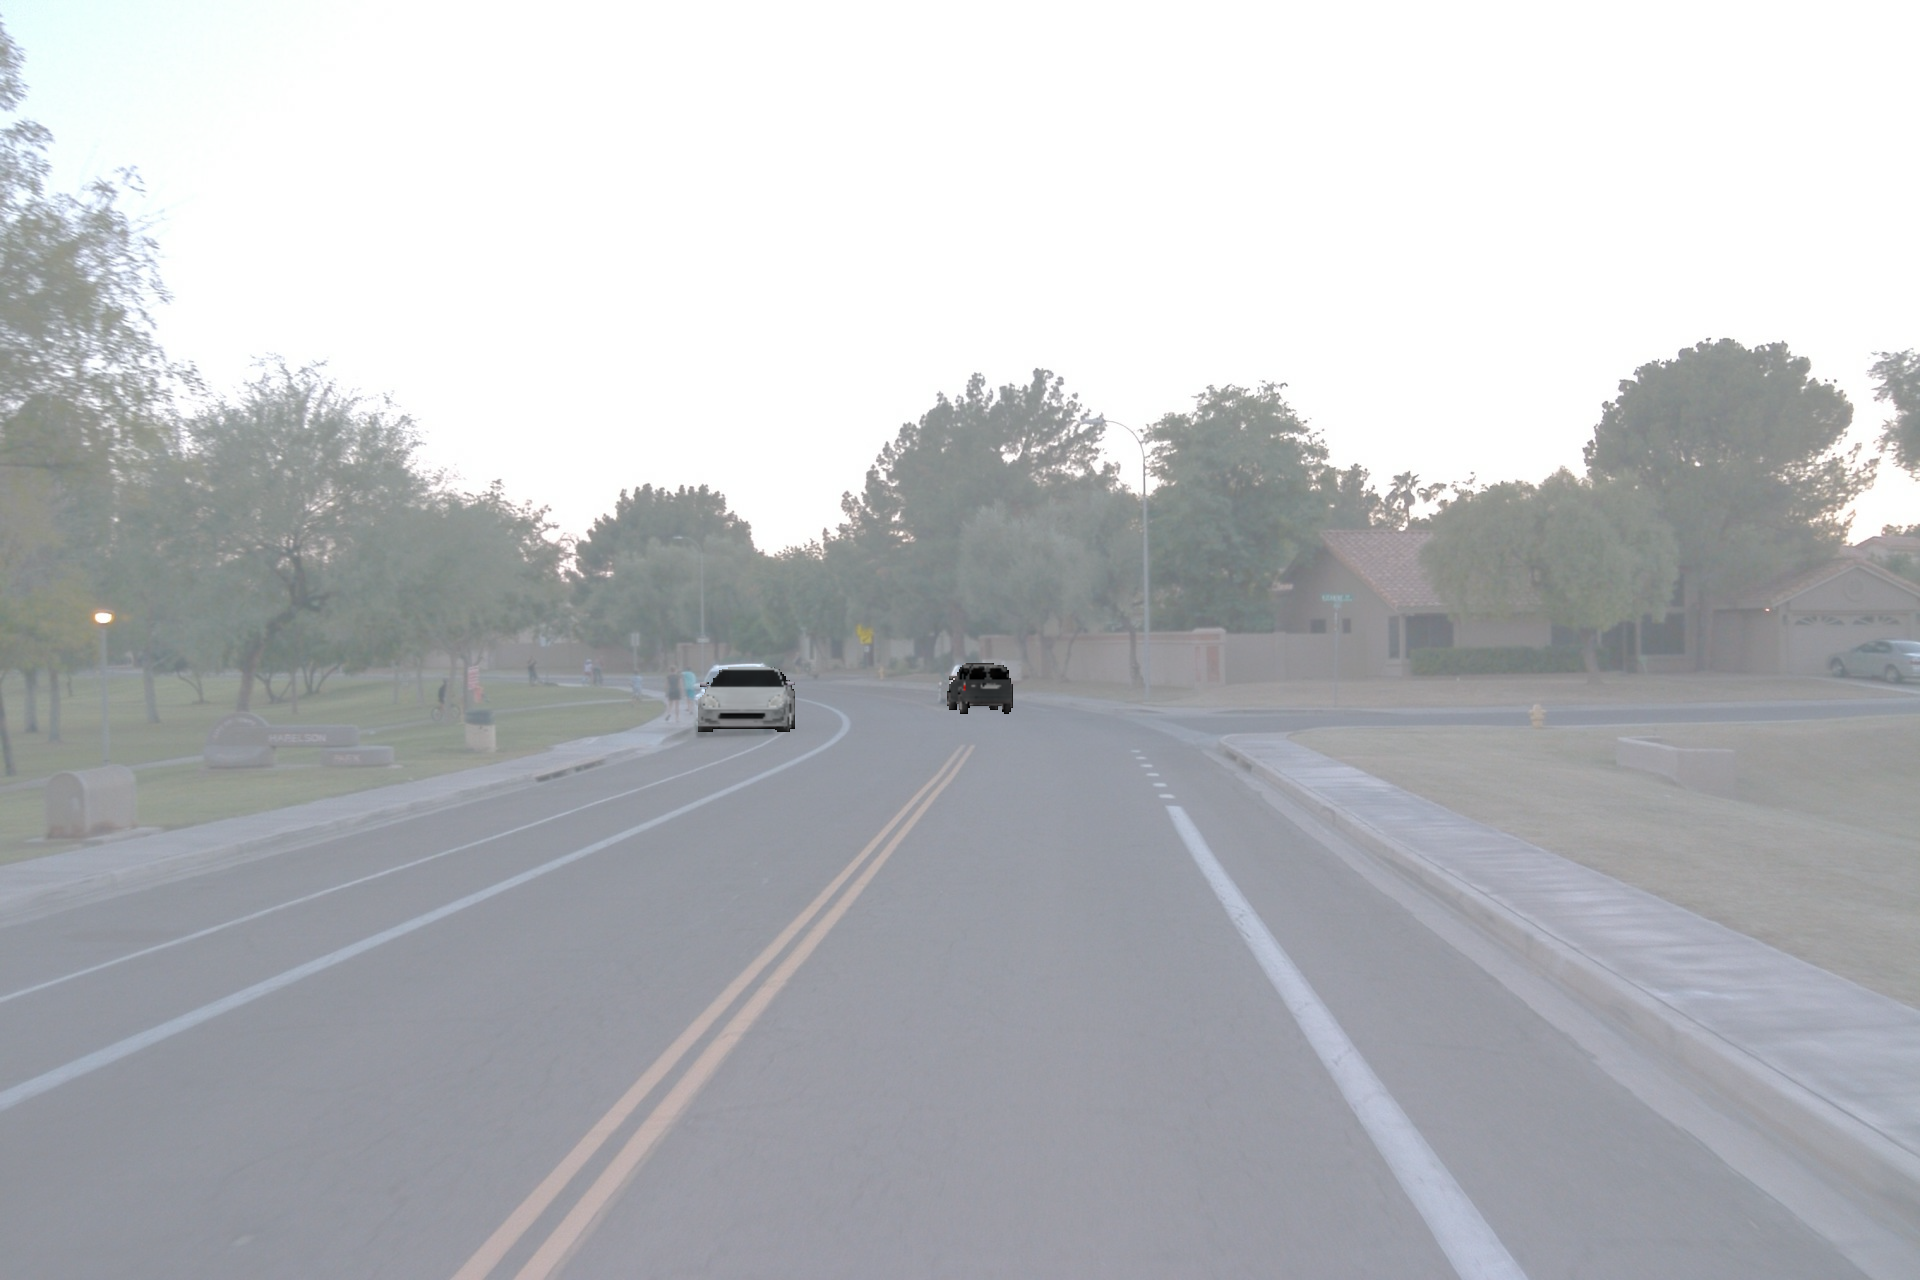
\includegraphics[width=.16\columnwidth, trim={22cm 16.68cm 30cm 18cm},clip]{fig/rebuttal_optimization/sched/82_60_shed.png}&
    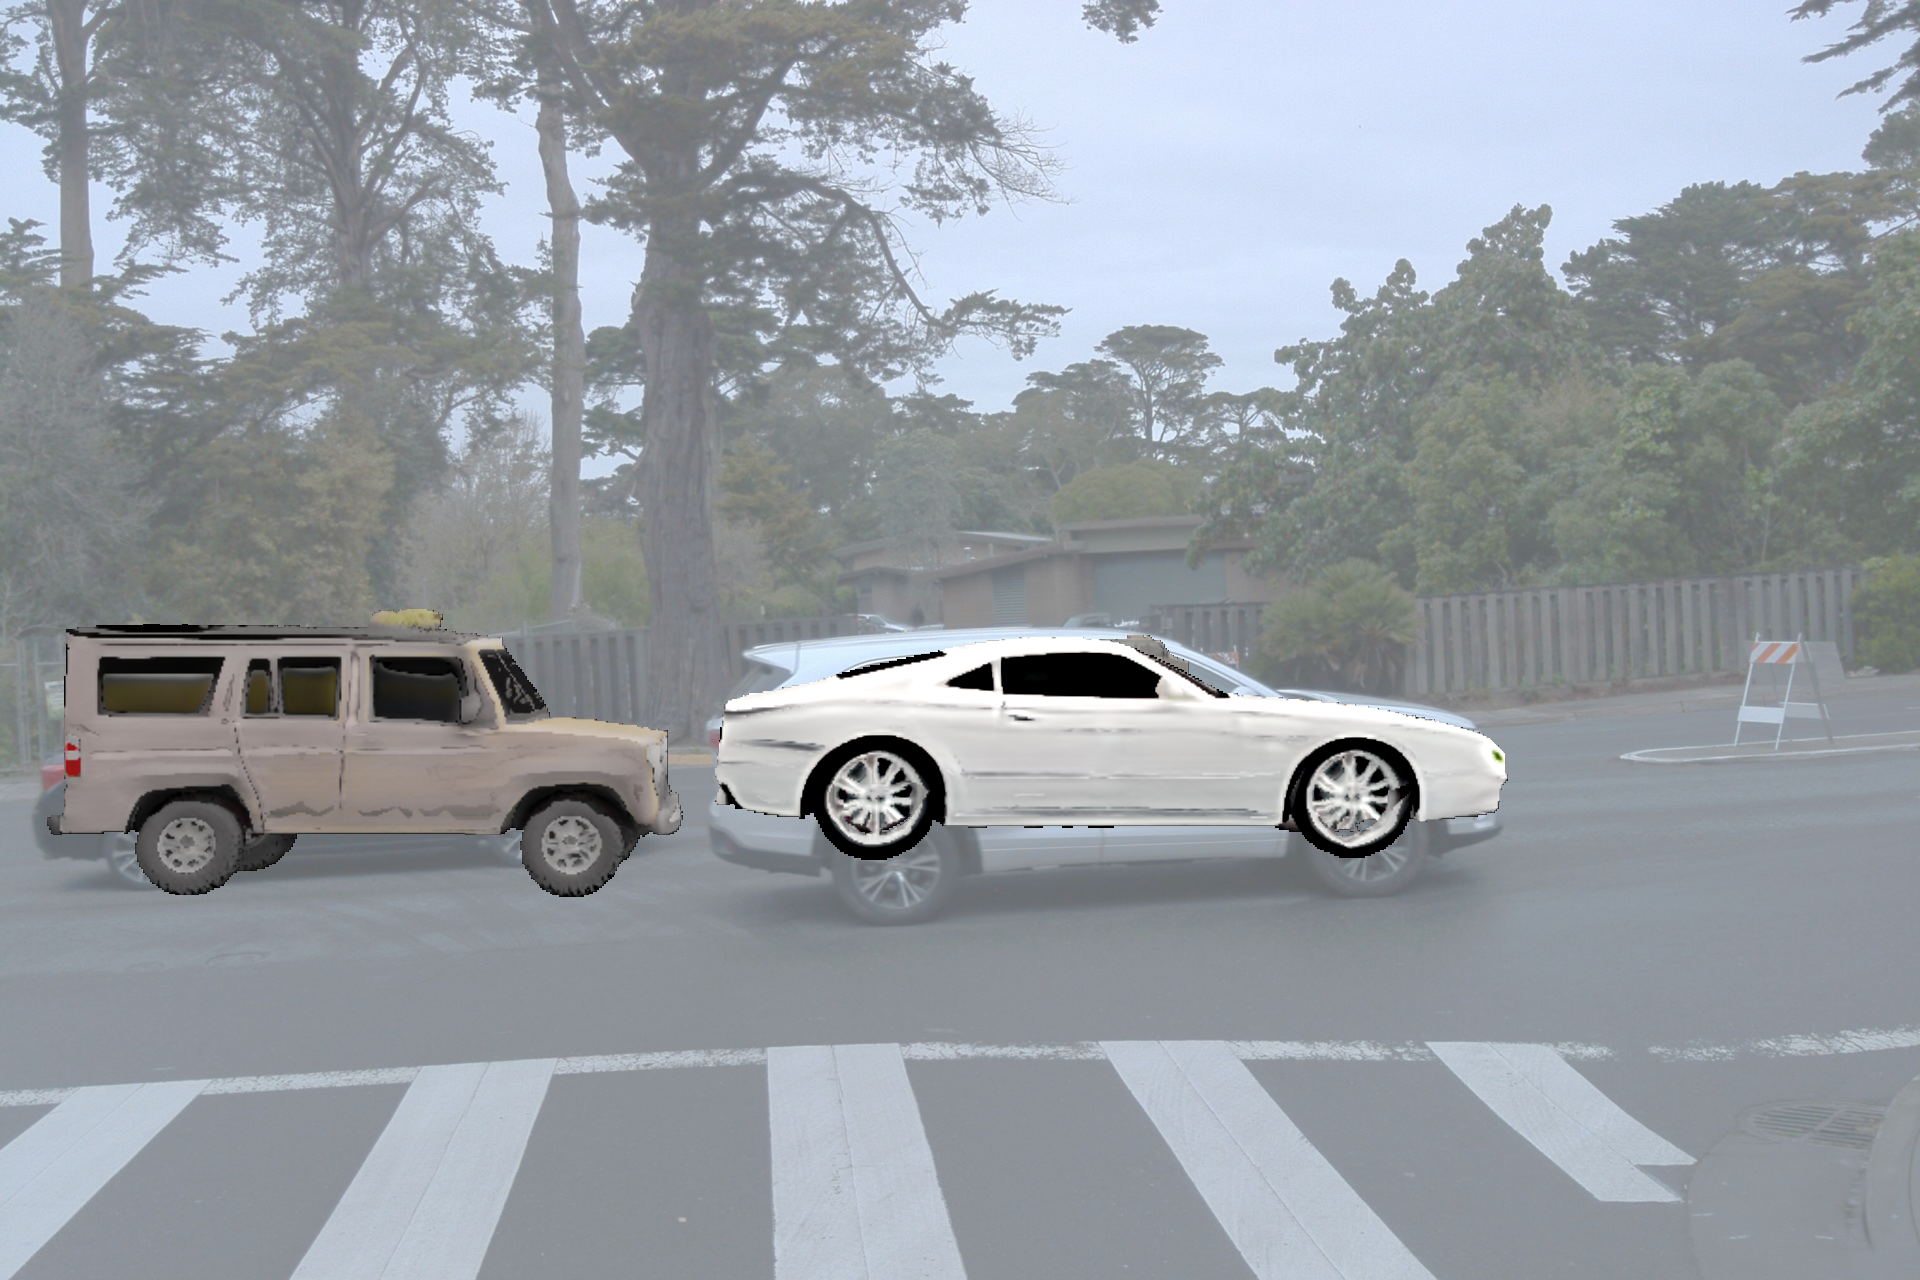
\includegraphics[width=.16\columnwidth, trim={0cm 0cm 0cm 0cm},clip]{fig/rebuttal_optimization/no_sched/11_102_no_sched.png}&    	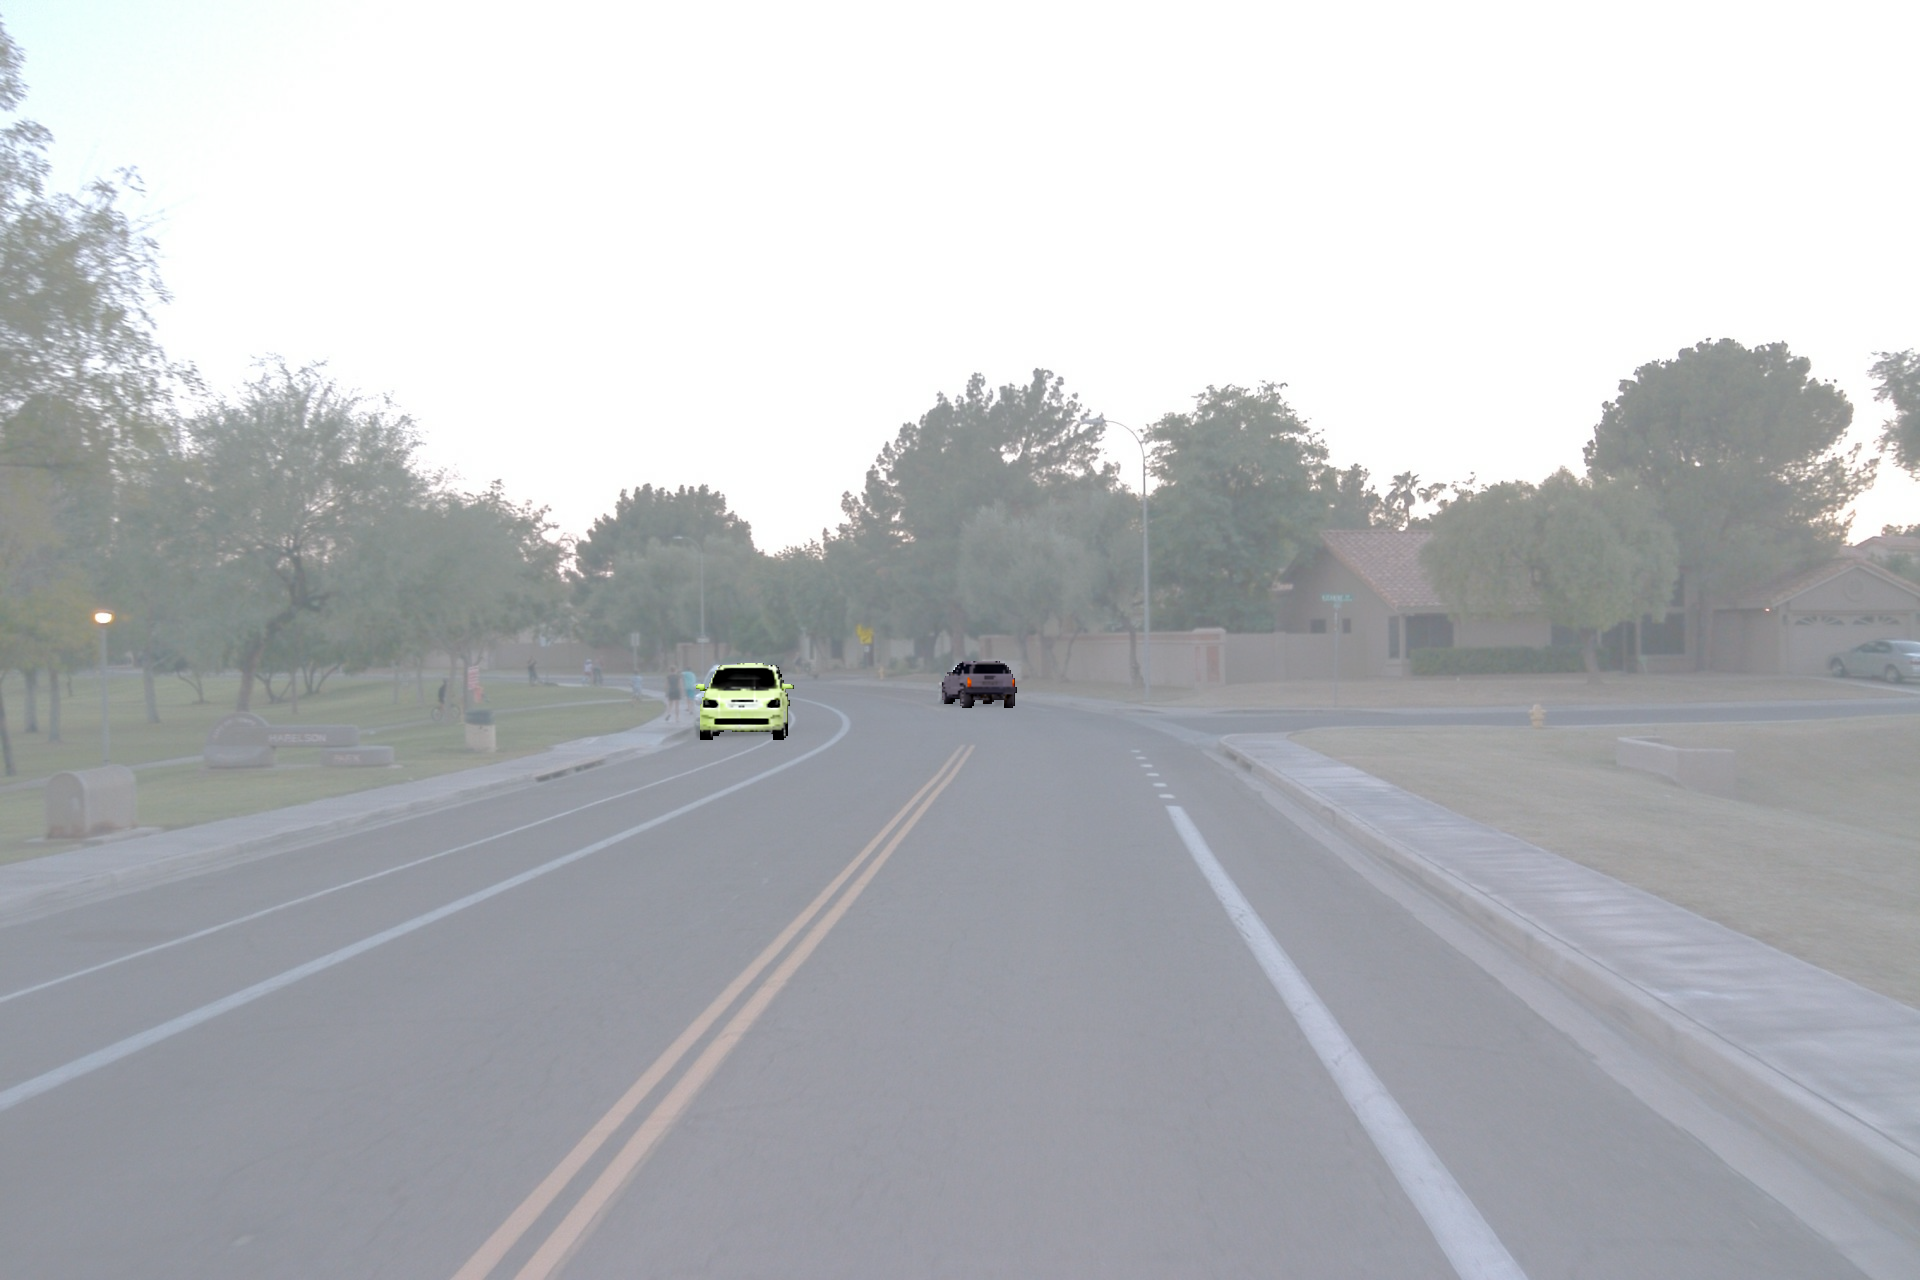
\includegraphics[width=.16\columnwidth, trim={22cm 16.68cm 30cm 18cm},clip]{fig/rebuttal_optimization/no_sched/82_60_no_shed.png}\\
    \end{tabular}
% }
    \vspace*{-6pt}
    \caption{\textbf{Effect of Optimization Schedule.} (a) observed image, (b) optimized generations using the proposed schedule in Sec.~\ref{sec:method}, (c) optimized generations using no schedule. \todo{move into table 2.}
 % , i.e. such that texture codes, shape codes, rotations, translations, and scales are all simultaneously optimized. The ground truth images are faded to show our rendered objects clearly. 
    % The bottom row shows images zoomed in to clearly show our rendered objects.
    % Our schedule allows for more stable optimization, with rendered objects more closely resembling the observed ones. 
} 
	\label{fig:opt_scheduler}
	% \vspace{-8pt}
\end{figure}